\documentclass{article}
\usepackage[utf8]{inputenc}
\usepackage[portuges]{babel}
\usepackage[a4paper, total={7in, 9in}]{geometry}
\usepackage{graphicx}
\usepackage{float}

\newcommand{\question}[1]{
    {\large \textbf{Q: #1}}
    \\
}

\newcommand{\titleRule}{
    \rule{\linewidth}{0.5mm} \\ [0.25cm]
}

\begin{document}

\begin{titlepage}
    \center
    \begin{figure}[H]
        \centering
        
\includegraphics[width=4cm]{UM_EENG.jpg}
    \end{figure}
    \textsc{\LARGE Universidade do Minho} \\ [1.5cm]
    \textsc{\Large Mestrado Integrado em Engenharia Informática} \\ [0.5cm]
    \textsc{\large Processamento de Dados com Streams de Java} \\ [0.5cm]

    \titleRule
    {\huge \bfseries Universal Time and Date Calculator}
    \titleRule
    
    João Pedro Ferreira Vieira A78468 \\
    Miguel Miranda Quaresma A77049 \\
    Simão Paulo Leal Barbosa A77689 \\[0.25cm]

    \today
\end{titlepage}

\newpage

\tableofcontents

\newpage

\section{Introdução}
O desenvolvimento de aplicações no contexto atual exige o recurso a técnicas que permitam não só gerir a sua complexidade, mas também garantir a robustez das mesmas.
\newline
Uma das técnicas empregadas para este fim consiste no uso de arquiteturas de software que definam, de forma clara, a estrutura das aplicações a um nível elevado.
\newline
Destas arquiteturas o \textbf{MVC}(Model-View-Controller) destaca-se como uma das mais utilizadas, pela sua clareza e modularidade, permitindo desenvolver os componentes integrantes da aplicação conhecendo apenas a sua API. Esta modularidade permite ainda identificar pontos de falha, facilitando a manutenção da aplicação.
\newline
A aplicação desenvolvida com recurso a esta arquitetura consiste numa ferramenta que apresenta um conjunto de funcionalidades no domínio temporal, apresentando três modos de funcionamento principais.

\newpage

\section{Arquitetura e Implementação}
Dadas as caraterísticas da aplicação (3 modos de funcionamento; menus baseados em texto; etc) a arquitetura considerada para o desenvolvimento da mesma foi MVC. 
Neste sentido foram identificadas as classes que pertenciam a cada um dos grupos(de componentes) caraterísticos desta arquitetura.
De seguida, para garantir uniformidade entre componentes do mesmo grupo, e aplicando a filosofia de desenvolvimento orientado a interfaces, foram desenvolvidas duas interfaces: \texttt{ControllerInterface} e \texttt{ViewInterface} para os grupos \texttt{Controller} e \texttt{View} respetivamente.

\subsection{Controllers}
Os Controllers são responsáveis pela ligação entre a camada de dados(Model) e a interface com o utilizador(View). 
A aplicação é então constituída por 4 controladores:
\begin{itemize}
    \item UTDCController
    \item DateTimeModeController
    \item ManagementController
    \item TimeZoneController
\end{itemize}
Como foi referido anteriormente, todos os controladores implementam a interface \texttt{ControllerInterface} que apresenta a seguinte API:
\begin{verbatim}
    void setView(ViewInterface v);
    void setModel(UTDCModel m);
    void startFlow(); 
\end{verbatim}

O \texttt{UTDCController} funciona como gestor dos modos de funcionamento, comutando entre os restantes (sub)controladores, conforme o 
modo pretendido pelo utilizador:

\begin{verbatim}
    public void startFlow(){
        Menu menu = view.getMenu(1);
        String opcao;
        do{
            menu.show();
            opcao = Input.lerString().toUpperCase();
            switch (opcao){
                case "D":
                    this.dateTimeController.startFlow();
                    break;
                case "M":
                    this.managementController.startFlow();
                    break;
                case "T":
                    this.timeZoneController.startFlow();
                    break;
                case "E":
                    break;
                default:
                    System.out.println("Invalid option!");
                    break;
            }
        } while (!opcao.equals("E"));
    }
\end{verbatim}

Como já foi referido, todos os Controladores implementam o método \texttt{startFlow} que é responsável por apresentar as funcionalidades disponibilizadas por um
dado modo(\texttt{Controller}) e, consoante a opção escolhida é invocado o método que permite obter o resultado pretendido.

\subsection{Views}
As \texttt{Views} são responsáveis por apresentar e recolher dados do utilizador, funcionando como o ponto de interação do mesmo com o sistema/aplicação.
Esta caraterística motivou a criação de 4 vistas distintas, apresentado todas a mesma API, recorrendo para isso à interface \texttt{ViewInterface}:
\begin{verbatim}
    public Menus getMenusUTDC();
    public void setMenusUTDC(Menus m);
    public Menu getMenu(int indice);
    public Menus initView();
    public void printColletion(String header, Collection<String> values); 
\end{verbatim}

As vistas:
\begin{itemize}
    \item UTDCView
    \item DateTimeView
    \item ManagementView
    \item TimeZoneView
\end{itemize}
foram desenvolvidas seguindo a mesma filosofia usada nos controladores, mapeando uma vista num modo funcionamento, com todos os sub-menus de um dado modo delegados na vista correspondente. Mais uma vez, a vista \texttt{UTDCView} corresponde ao menu principal, onde são apresentados os três modos de funcionamento disponíveis.

\subsection{Models}
Os \texttt{Models} correspondem à camada de dados da aplicação, sendo que qualquer operação sobre estes deve ser realizada nesta camada, cabendo apenas aos controladores requisitar os dados e à vista apresentá-los.
No contexto da aplicação a desenvolver, foi identificado como entidade relevante um evento no modo agenda, sendo que esta entidade deve armazenar todos os dados úteis à representação do mesmo, de acordo com a funcionalidade esperada de uma agenda. Como tal foram identificados os seguintes atributos:
\begin{verbatim}
    private LocalDateTime date;
    private Duration duration;
    List<String> people_envolved;
    String title;
    String description;
    String local;
    DayOfWeek dayOfWeek;
\end{verbatim}

Para poder representar a informação referente a um dado evento foram desenvolvidos dois métodos que permitem consultar dois esta mesma informação, diferindo apenas na quantidade de informação.
O método \texttt{public String getInfoShort();} permite consultar um resumo das caraterísticas do evento em causa, sendo usado quando é necessário listar um conjunto de eventos, por forma a apresentar apenas a informação fundamental referente aos mesmos.
O método \texttt{public String getInfoDetails();} é usado para obter a descrição completa do evento, sendo útil quando um utilizador pretende, por exemplo, alterar os dados de um evento.

Adicionalmente, foi desenvolvido o modelo \texttt{User} que permite a criação de utilizadores
associados a uma dada agenda. Este modelo apresenta os seguintes atributos:
\begin{verbatim}
    private String username;
    private String name;
    private String password;    
\end{verbatim}

Para consultar a sua agenda o utilizador deve inserir o seu \textit{username} e a sua \textit{password}.

Para permitir a manipulação de eventos e de utilizadores a classe \texttt{UTDCModel} armazena uma lista de eventos bem como os utilizadores que registaram esses eventos.

\begin{verbatim}
    //Map<username,eventos>
    Map<String,List<EventModel>> events;
    //Map<username,user>
    Map<String,User> users;
\end{verbatim}

Esta classe implementa diversos métodos fundamentais ao funcionamento da aplicação:
\begin{description}
    \item [iniciar sessão:]\texttt{ public int login(String username, String password);} 
    \item [registar utilizadores:]\texttt{public int registUser(String username, String name, String password);}
    \item [adicionar eventos:]\texttt{public void addEvent(String username, EventModel em);} 
    \item [remover eventos:]\texttt{public void removeEvent(String username, EventModel em);}
    \item [consultar eventos:]\texttt{public List<EventModel> getEventsRaw(String username);}
\end{description}

\subsection{Validação de Input}
Um dos requisitos mais críticos de uma aplicação que compreenda interação com utilizadores é a validação dos dados introduzidos pelos mesmos. Esta necessidade
é motivada pelos diversos lapsos que podem ocorrer na inserção de dados ou mesmo devido a utilizadores mal intencionados que insiram dados com o objetivo
de alterar o comportamento da aplicação. Como tal, a \textbf{UTDCApp} recorre à classe \texttt{Input} que disponibiliza um conjunto de métodos que permitem 
ler dados do \textit{standard input} e efetua a validação dos mesmos tendo em conta o tipo dos dados a ser lidos. 
Como é possível inferir pela natureza da aplicação, os dados lidos serão de cariz temporal, tanto referentes a datas, como a \textit{timestamps}, como tal
é importante destacar os seguintes métodos presentes na classe \texttt{Input}:

\begin{verbatim}
    public static LocalDate lerDate(String format); 
    public static LocalDateTime lerDateTime(String format); 
    public static LocalTime lerTime(String format); 
    public static DayOfWeek lerWeekDay(); 
\end{verbatim}

A formatação de valores temporais, que é feito com recurso à classe \texttt{DateFormat} que permite especificar o formato pretendido, 
realizando o \textit{parsing} do valor lido tendo o mesmo em conta. 
Os métodos que devolvem objetos do tipo \texttt{lerDate, lerDateTime e lerTime}) recebem como argumento o formato pretendido.
Visto ser possível introduzir três tipos diferentes de dados temporais, quando o utilizador é solicitado um destes tipos
é-lhe previamente indicado o formato esperado, sendo ainda dada possibilidade de escolher entre os mesmos quando aplicável:

\begin{figure}[H]
    \centering
    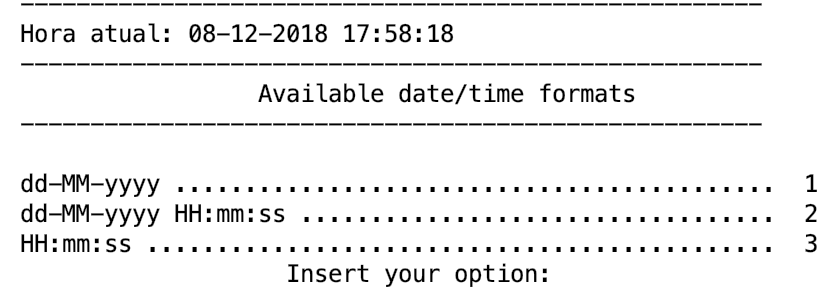
\includegraphics[width=8.5cm]{date_formats.png}
\end{figure}

\textbf{N.B.:} O uso frequente dos formatos esperados para um destes tipos (\texttt{LocalDate, LocalDateTime, LocalTime}) motivou a criação de três variáveis 
com os modificadores \texttt{static final} na classe \texttt{UTDCController}.

\begin{verbatim}
    protected static final String local_date_format = "dd-MM-yyyy";
    protected static final String local_time_date_format = "dd-MM-yyyy HH:mm:ss";
    protected static final String local_time_format = "HH:mm:ss"; 
\end{verbatim}

\subsection{Funcionalidades Adicionais}
Por forma a acomodar uma expansão futura do domínio de uso da aplicação desenvolvida, foi implementado um sistema de gestão de utilizadores
que permite associar um dado utilizador a uma lista de eventos (agenda):
\begin{verbatim}
    //Map<username,eventos>
    Map<String,List<EventModel>> events;
    //Map<username,user>
    Map<String,User> users;
\end{verbatim}

Quando é selecionado o modo \textit{Slot Management}, o utilizador deve fornecer o seu \textit{username} e \textit{password} para carregar a sua agenda ou registar-se na plataforma para poder usufruir da funcionalidade.
De seguida, todos os eventos criados nessa sessão(conta) bem como a consulta dos mesmos é feita no conjunto de eventos associado ao utilizador atual:
\begin{verbatim}
   List<String> event_info = this.model.getShortEvents(this.username);     
   ...
   List<String> future_info = this.model.getFutureEvents(this.username,after);
   ...
   List<String> events_date = this.model.getEventsTimeInterval(this.username,start,end);
   ...
   List<String> past_info = this.model.getPastEvents(this.username,before);
   ....
   List<String> events_weekday = this.model.getEventsByDayOfWeek(this.username,w_day);
   ...
\end{verbatim}

Como foi referido ao falar da classe \texttt{UTDCModel}, o mecanismo implementado impede ainda que utilizadores manipulem eventos que não sejam "seus".

\newpage

\section{Manual de utilização}
A aplicação UTDC apresenta um conjunto de funcionalidades para manipular/trabalhar dados temporais, apresentando 3 modos principais que se distinguem pelo tipo de operações que disponibilizam.
O menu inicial apresenta 3 modos:

\begin{figure}[H]
    \centering
    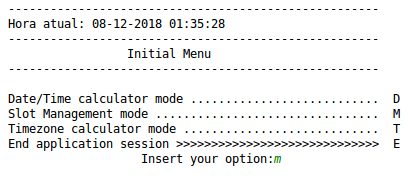
\includegraphics[width=8.5cm]{menu_inicial.png}
    \caption{Menu inicial da plataforma \textit{UTDC}}
\end{figure}

O utilizador pode selecionar o modo pretendido inserindo a letra correspondente.
\subsection{Modos de Funcionamento}

\subsubsection{Date/Time calculator mode}
Este modo apresenta as seguintes funcionalidades:

\begin{figure}[H]
    \centering
    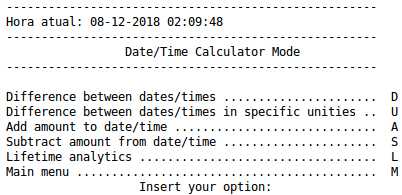
\includegraphics[width=8.5cm]{date_time.png}
    \caption{Funcionalidades do modo Date/Time}
\end{figure}

\begin{itemize}
    \item \textbf{Difference between dates/times} - Calcula a diferença entre duas datas/tempos inseridas, sendo estas datas/tempos divididos em 3 possíveis formatos: "dia-mês-ano" ,  "dia-mês-ano hora:minuto:segundo" e\\ "hora:minuto:segundo". Por exemplo, a diferença entre "12-10-2018" e "14-12-2020" é "2 Years 2 Months 2 Days".
    \item \textbf{Difference between dates/times in specific unities} - Calcula a diferença entre duas datas/tempos (com os mesmos formatos anteriores) inseridas, em unidades de tempo especificas, escolhidas pelo utilizador. Por exemplo, a diferença entre "12-10-2018" e "14-12-2020" em dias e semanas é "794 Days 113 Weeks". 
    \item \textbf{Add amount to date/time} - Adiciona um intervalo de tempo escolhido pelo utilizador( com diversas opções de unidades de tempo) para adicionar a uma data inserida pelo mesmo. Por exemplo, se for adicionado 1 mês e 1 dia  á data "10-12-2018" , o resultado obtido é  "11-01-2019"
    \item \textbf{Subtract amount from date/time} - Função inversa á anterior, subtrai em vez de somar um intervalo de tempo.
    \item \textbf{Lifetime analytics} - Depois de  inserida a data de nascimento do utilizador, apresenta diferentes opções de estatísticas sobre esta:
        \begin{itemize}
        \item \textbf{Age at given date} - Indica a idade do utilizador numa data inserida pelo mesmo, esta pode ser apresentado em diversos formatos
        \item \textbf{Day of week of day of next birthday} - Apresenta o dia da semana do próximo aniversário do utilizador, por exemplo: "Your next birthday (16-11-2019) is in a Saturday"
        \item \textbf{Birthday-Weekday percentage distribuition} - Apresenta a distribuição aniversário/dia da semana do utilizador  
        \item \textbf{Amount of leap years in lifetime} - Apresenta os anos Bissextos que o utilizador já vivenciou
        \end{itemize}
        
    
\end{itemize}

\subsubsection{Slot Management mode}

Este modo permite ao utilizador marcar e consultar eventos marcados na sua agenda\newline
Este modo inicia-se com a opção de fazer autenticação com um dado utilizador já criado ou efetuar registo no sistema.\newline

\begin{figure}[H]
    \centering
    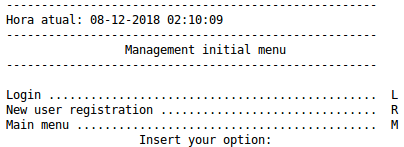
\includegraphics[width=8.5cm]{management_login.png}
    \caption{Autenticação ou registo de utilizador}
\end{figure}

Apartir do momento em que o \textit{login} é efetuado são disponibilizadas ao utilizador as seguintas funcionalidades:

\begin{figure}[H]
    \centering
    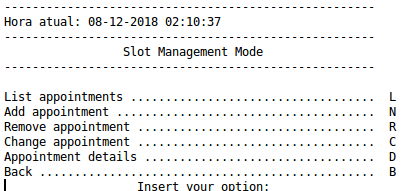
\includegraphics[width=8.5cm]{management.png}
    \caption{Menu inicial da plataforma \textit{UTDC}}
\end{figure}

\begin{itemize}
    \item \textbf{List appointments} - Mostra os eventos marcados pelo utilizador com 5 tipos de procuras diferentes:
        \begin{itemize}
            \item \textbf{Check all events} - Mostra uma breve descrição de todos os eventos que o utilizador registou
            \item \textbf{Check future events} - Apresenta os eventos futuros ordenados pelas suas datas
            \item \textbf{Check events in a given date} - Verificar quais os eventos que estão marcados num dado dia
            \item \textbf{Check events in x amount of time} - Mostrar os eventos que se encontram num intervalo de tempo definido pelo utilizador
            \item \textbf{Check past events} Mostra os eventos que já se realizaram ordenados por data
        \end{itemize}
    \item \textbf{Add appointment} - Regista um novo evento na agenda do utilizador
    \item \textbf{Remove appointment} - Permite remover um dado evento na agenda do utilizador
    \item \textbf{Change appointment} - Dá a possibilidade de alterar os dados de um dado evento
    \item \textbf{Appointment details} - Mostra informação pormenorizada de um evento procurado pelo utilizador
\end{itemize}

\subsubsection{Timezone calculator mode}
Este modo apresenta as seguintes funcionalidades:

\begin{figure}[H]
    \centering
    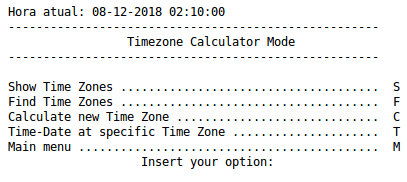
\includegraphics[width=8.5cm]{timezone.png}
    \caption{Funcionalidades do modo \textit{Timezone}}
\end{figure}

\begin{itemize}
    \item \textbf{Show Time Zones} - Imprime todas as Time Zones disponíveis para posterior utilização
    \item \textbf{Find Time Zones} - Encontra Time Zones por comparação com uma palavra inserida
    \item \textbf{Calculate new Time Zone} - Converte uma data de uma Time Zone para outra, dividindo-se assim em 3 opções:
        \begin{itemize}
        \item \textbf{Your time zone    --\textgreater  Custom time zone} - Converte da time zone atual do utilizador para outra que será inserida
        \item \textbf{Custom time zone  --\textgreater   Your time zone} - Converte de uma time zone inserida para a time zone atual do utilizador
        \item \textbf{Custom time zone  --\textgreater   Custom time zone} - Converte de uma Time Zone para outra, ambas inseridas pelo utilizador
        \end{itemize}
    \item \textbf{Time-Date at specific Time Zone} - Data e tempo atuais em uma Time Zone inserida pelo utilizador
\end{itemize}

\newpage

\section{Conclusão}
Como foi possível observar, o sistema desenvolvido pode facilmente ser aplicado num contexto de mundo real, sendo que o facto de incluir várias 
funcionalidades no domínio de datas/tempo numa só aplicação é conseguido através da Date-Time API disponibilizada pela linguagem Java.
Adicionalmente, é claro que o uso da arquitetura MVC agilizou de forma considerável o processo de desenvolvimento da aplicação ao permitir, numa
fase inicial, que os diversos componentes fossem desenvolvidos de forma independente e, consequentemente, permitiu identificar de maneira mais 
eficiente possíveis problemas com o comportamento da aplicação visto que as camadas que constituíam as mesma se encontravam logicamente divididas.

\end{document}